%% abtex2-modelo-slides.tex, v-1.0 gfabinhomat
%% Copyright 2012-2014 by abnTeX2 group at http://abntex2.googlecode.com/ 
%%
%% This work may be distributed and/or modified under the
%% conditions of the LaTeX Project Public License, either version 1.3
%% of this license or (at your option) any later version.
%% The latest version of this license is in
%%   http://www.latex-project.org/lppl.txt
%% and version 1.3 or later is part of all distributions of LaTeX
%% version 2005/12/01 or later.
%%
%% This work has the LPPL maintenance status `maintained'.
%% 
%% The Current Maintainer of this work is Fábio Rodrigues Silva, 
%% member of abnTeX2 team, led by Lauro César Araujo. 
%% Further information are available on 
%% http://abntex2.googlecode.com/
%%
%% This work consists of the files abntex2-modelo-slides.tex, 
%% abntex2-modelo-references.bib and abntex2-modelo-marca.pdf
%%
%% Modelo desenvolvido por Fábio Rodrigues Silva (gfabinhomat@gmail.com)
%% Mais informações podem ser obtidas no guia do usuário Beamer 
%% (http://linorg.usp.br/CTAN/macros/latex/contrib/beamer/doc/beameruserguide.pdf)
%% Informações rápidas podem ser acessadas em http://en.wikibooks.org/wiki/LaTeX/Presentations


% Apresentações em widescreen. Outros valores possíveis: 1610, 149, 54, 43 e 32.
% Por padrão, as apresentações são no formato 4:3 (sem o aspectratio).
\documentclass[aspectratio=169]{beamer}	 	

\titulo{Improvisações de códigos para análise de um algoritmo tonal no \emph{A Study in Keith} (2009) de Andrew Sorensen}
\autor{Guilherme Martins Lunhani}

\instituicao{Universidade Federal de Juiz De Fora -- UFJF
  \par
  Instituto de Artes e Design -- IAD
  \par
  Programa de Pós-Graduação em Artes Visuais, Música e Tecnologia}

\orientador[Orientador: ]{Prof. Dr. Luiz Eduardo Castelões}

\data{\today}

% \changes{Versão inicial }{2013/07/22 }{v0.0.3}
\tipotrabalho{Tese (Mestrado)}

% O preambulo deve conter o tipo do trabalho, o objetivo, 
% o nome da instituição e a área de concentração 
\preambulo{Dissertação corrigida para a banca de qualificação no Programa Mestrado em Artes, Cultura e Linguagens do Instituto de Artes e Design da Universidade Federal de Juiz de Fora (UFJF), linha de Artes Visuais, Musica e Tecnologia.}
%\EnableCrossrefs
%\CodelineIndex
%\RecordChanges

% ---
% Configurações de aparência do PDF final

% alterando o aspecto da cor azul
\definecolor{blue}{RGB}{41,5,195}

% informações do PDF
\makeatletter
\hypersetup{
     	%pagebackref=true,
		pdftitle={\@title}, 
		pdfauthor={\@author},
    	pdfsubject={\imprimirpreambulo},
	    pdfcreator={LaTeX with abnTeX2},
		pdfkeywords={abnt}{latex}{abntex}{abntex2}{trabalho acadêmico}, 
		colorlinks=true,       		% false: boxed links; true: colored links
    	linkcolor=blue,          	% color of internal links
    	citecolor=blue,        		% color of links to bibliography
    	filecolor=magenta,      		% color of file links
		urlcolor=blue,
		bookmarksdepth=4
}
\makeatother

%\newcommand{\todosautoresdelivecoding}{\begin{inparaenum}[]\item \citeonline{collins_live_2003},\item \citeonline{collins_generative_2003},\item \citeonline{collins_live_2003-1},\item \citeonline{wang_--fly_2004},\item \citeonline{ward_live_2004},\item \citeonline{blackwell_programming_2005},\item \citeonline{collins_live_2007},\item \citeonline{griffiths_fluxus:_2008},\item \citeonline{mclean_patterns_2009},\item \citeonline{rohrhuber_improvising_2009},\item \citeonline{mclean_visualisation_2010},\item \citeonline{magnusson_algorithms_2011},\item \citeonline{mccallum_show_2011},\item \citeonline{magnusson_herding_2014},\item \citeonline{magnusson_scoring_2014},\item \citeonline{collins_algorave:_2014},\item \citeonline{sorensen_livecodings_2014}\end{inparaenum}}
% --- 
% Espaçamentos entre linhas e parágrafos 
% --- 

% O tamanho do parágrafo é dado por:
\setlength{\parindent}{1.3cm}

% Controle do espaçamento entre um parágrafo e outro:
\setlength{\parskip}{0.2cm}  % tente também \onelineskip

% ---
% compila o indice
% ---
\makeindex

% ---
% Pacotes básicos 
% ---
\usepackage[utf8]{inputenc}		% Codificacao do documento (conversão automática dos acentos)
\usepackage{lmodern}			% Usa a fonte Latin Modern			
\usepackage[T1]{fontenc}		% Selecao de codigos de fonte.
\usepackage{lastpage}			% Usado pela Ficha catalográfica
\usepackage{indentfirst}		% Indenta o primeiro parágrafo de cada seção.
\usepackage{color}				% Controle das cores
\usepackage{graphicx}			% Inclusão de gráficos
\usepackage{wallpaper}			% inclusao de imagens deslocadas
\usepackage{microtype} 			% para melhorias de justificação
\usepackage{url}
\usepackage[table,xcdraw]{xcolor}
\usepackage{tabularx}
\usepackage{minted}
\usepackage{amsmath,amssymb}
\usepackage{framed}
\usepackage[amsmath,framed]{ntheorem}
\usepackage{pdfpages}

% ---
		
% ---
% Pacotes adicionais, usados apenas no âmbito do Modelo Canônico do abnteX2
% ---
\usepackage{lipsum}				% para geração de dummy text
% ---

%---
% Pacote para listas em uma linha
%---
\usepackage{paralist}

% ---
% Epigrade
% ---
\usepackage{epigraph}

% Front end para amsthm (\declaretheorem)
\usepackage{thmtools}    

% ---
% Pacotes de citações
% ---
\usepackage[brazilian,hyperpageref]{backref}	 % Paginas com as citações na bibl
\usepackage[alf]{abntex2cite}	% Citações padrão ABNT

%TODO
\usepackage[colorinlistoftodos]{todonotes}
%\usepackage{ntheorem}

\usepackage{tablefootnote}


%%%%%%%%%%% syntax highlight %%%%%%%%%%%%%%%%%%%%%%%%%%%%%%%%%%%%%%%%%%%%%%%%%%%%%
\usepackage{listings}
\definecolor{maroon}{rgb}{0.5,0,0}
\definecolor{darkgreen}{rgb}{0,0.5,0}
\definecolor{deepblue}{rgb}{0,0,0.5}
\definecolor{deepred}{rgb}{0.6,0,0}
\definecolor{purple}{rgb}{0.5,0,0.5}
\definecolor{deepgreen}{rgb}{0,0.5,0}
%%%%%%%%%%%%%%%%%%%%%%%%%%%%%%%%%%%%%%%%%%%%%%%%%%%%%%% 

\usepackage{tikz}
\tikzset{
  treenode/.style = {shape=rectangle, rounded corners,
                     draw, align=center,
                     top color=white, bottom color=blue!20},
  root/.style     = {treenode, font=\Large, bottom color=red!30},
  env/.style      = {treenode, font=\ttfamily\normalsize},
  dummy/.style    = {circle,draw}
}


% ----------------- INÍCIO DO DOCUMENTO --------------------------------------
\begin{document}

% ----------------- NOVO SLIDE --------------------------------
\input{./titulo}

% ----------------- NOVO SLIDE --------------------------------
\begin{frame}{Sumário}
\tableofcontents
\end{frame}

% ----------------- NOVO SLIDE --------------------------------
\section{Preambulo}
\begin{frame}{Preâmbulo}
O tema da improvisação de códigos, como um universo de conceitos, surgiu de uma experiência com um código em linguagem \emph{python} (\url{https://www.python.org}), útil para gerar um mapa de termos, como ilustrado na figura abaixo.
\end{frame}

% ----------------- NOVO SLIDE --------------------------------
\begin{frame}{Preâmbulo}
\begin{figure}
\centering
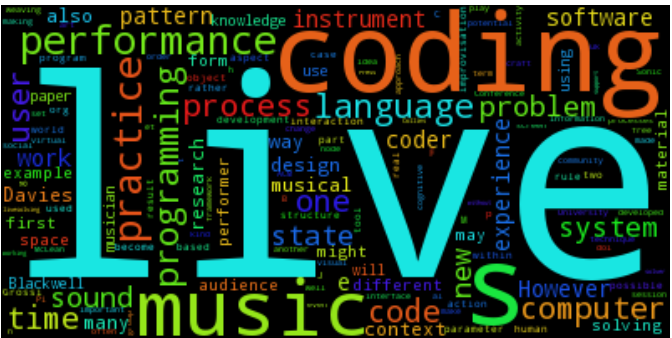
\includegraphics[scale=0.8]{imagens/nuvem.png}
\caption{Nuvem de palavras do \citeonline{ICLC2015},  1$^o$ Congresso Internacional de Live Coding. \textbf{Fonte}: autor.}
\label{fig:nuvemlivecoding}
\end{figure}
\end{frame}

\section{Introdução}
% ----------------- NOVO SLIDE --------------------------------
\begin{frame}{Introdução}
Metáfora:

Livecoding como venda de filosofias $\rightarrow$ Mercado emergente do conhecimento das artes computacionais.
\end{frame}

% ----------------- NOVO SLIDE --------------------------------
\begin{frame}{Introdução}
Metáfora:

Livecoding (improvisação de códigos) como venda de filosofias $\rightarrow$ Mercado emergente do conhecimento das artes computacionais.
\end{frame}

% ----------------- NOVO SLIDE --------------------------------
\begin{frame}{Introdução}
Abordagem do conhecimento das artes computacionais no \emph{Livecoding}:

• Conhecimento ortopédico $\rightarrow$ Universo de conceitos, bricolagem

• Razão indolente $\rightarrow$ metáforas e imagens mentais de uma improvisação de códigos são reduzidos como um objeto com diversas propriedades.

• Pensamento abissal $\rightarrow$ divisão dos que praticam o \emph{Livecoding} do ambiente europeu, e dos que não praticam fora do contexto europeu.
\end{frame}

% ----------------- NOVO SLIDE --------------------------------
\begin{frame}{Introdução}
Abordagem do conhecimento das artes computacionais no \emph{Livecoding}:
• Universo de conceitos
\end{frame}

\begin{frame}{Objetivo}
• Investigar um Universo de Conceitos sobre a \emph{improvisação de códigos} (\emph{live coding});

• Investigar um Espaço de Conceitos, historicamente restrito, sobre a improvisação de códigos;

• Investigar um método de análise/criação para uma improvisação de códigos;

• Investigar um Espaço Conceitual de uma improvisação de códigos, \emph{A Study in Keith} (2009) de Andrew Sorensen, e seu algoritmo musical em um ciclo de transformação.
\end{frame}

\section{Definições de base da Improvisação de códigos}
% ----------------- NOVO SLIDE --------------------------------
\begin{frame}{Definições de base da Improvisação de códigos}
\emph{Live coding} é uma técnica artística de improvisação. Pode ser empregada em muitos contextos diferentes de performance: dança, música, imagens em movimento e mesmo tecelagem. Eu concentrei minha atenção no lado musical, que parece ser o mais proeminente \cite[p.~117]{mori_analysing_2015}
\end{frame}

% ----------------- NOVO SLIDE --------------------------------
\begin{frame}{Definições de base da Improvisação de códigos}
A definição denota a aplicação em qualquer outra área, não apenas como metáfora, mas como estratégia de gerenciamento de fluxos criativos, assistidos por computador
\end{frame}

% ----------------- NOVO SLIDE --------------------------------
\begin{frame}{Tecelagem}
O grupo \emph{Weaving codes} foi formado para  a \emph{(\ldots) investigação de padrões a partir das perspectivas de tecelagem e música, e através do desenvolvimento de uma linguagem de computador e código para descrever a construção de tecidos} \cite{griffths_weave_2015}
\end{frame}

% ----------------- NOVO SLIDE --------------------------------
\begin{frame}{Tecelagem}
\emph{Uma das idéias originais era combinar tecelagem e codificação em um cenário de atuação, ambos para fornecer uma forma de tornar a codificação ao vivo mais inclusiva com a tecelagem, e ao mesmo tempo esclarecer os processos de pensamentos digitais envolvolvidos na tecelagem (\ldots) Nossa audiência consistiu de pesquisadores de artesanato, biólogos antropológicos, arquitetos, designers de jogos e tecnólogos -- foi mais do que antecipamos! Alex e eu disponibilizamos alguns códigos de música do \emph{slub} para tecer, e minha parte favorita foi projetar a tecelagem ao vivo} \cite{griffths_weave_2015}.
\end{frame}

% ----------------- NOVO SLIDE --------------------------------
\defverbatim[colored]{\tecelagem}{
\begin{minted}[fontsize=\scriptsize]{cl}
(twist 3 4 5 14 15 16)
(weave-forward 3)
(twist 4 15)
(weave-forward 1)
(twist 4 8 11 15)

(repeat 2
 (weave-back 4)
 (twist 8 11)
 (weave-forward 2)
 (twist 9 10)
 (weave-forward 2)
 (twist 9 10)
 (weave-back 2)
 (twist 9 10)
 (weave-back 2)
 (twist 8 11)
 (weave-forward 4))
\end{minted}
}

\begin{frame}{Tecelagem}
\tecelagem
\end{frame}

% ----------------- NOVO SLIDE --------------------------------
\begin{frame}{Tecelagem}
\begin{figure}[!h]
    \centering
    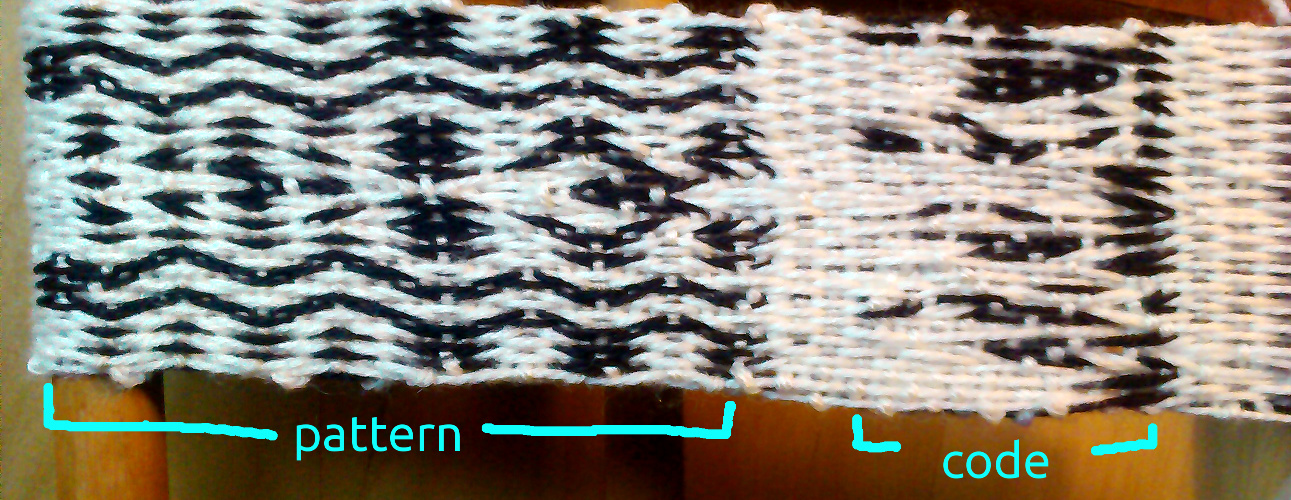
\includegraphics[scale=0.31]{imagens/weaving.jpg}
    \caption{Tecido resultante da prática \emph{Weaving code}. \textbf{Fonte}: \citeonline{griffths_weave2_2015}.}
  \label{fig:weaving}
\end{figure}
\end{frame}

% ----------------- NOVO SLIDE --------------------------------
\begin{frame}{Tecelagem}
• Apresentação de dois importantes personagens para o \emph{Livecoding}: Alex McLean e Dave Griffths (\emph{Slub})

• Observação de possíveis rituais de \emph{livecoding}, como apresentação artística informal/formal.
\end{frame}

% ----------------- NOVO SLIDE --------------------------------
\begin{frame}{Tecelagem}
\begin{figure}[h]
  \centering
  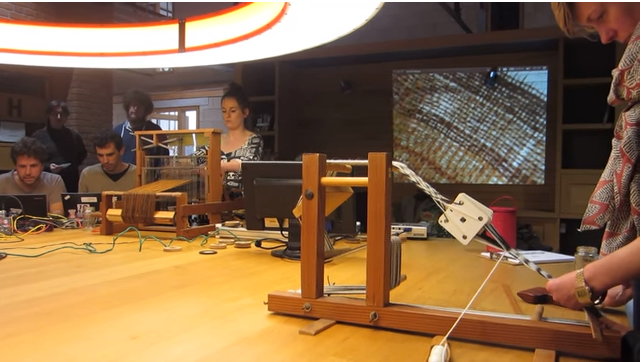
\includegraphics[scale=0.5]{imagens/weaving.png}
  \caption{Performance no Foam Kernow. \textbf{Fonte}: \citeonline{griffths_weave_2015}.}
  \label{fig:weavecoding}
\end{figure}
\end{frame}

% ----------------- NOVO SLIDE --------------------------------
\begin{frame}{Slub}
A banda \emph{Slub} começou em 2000, como uma colaboração entre Adrian Ward e Alex McLean. A premissa do duo era utilizar a atividade de programação para realização de uma Música Eletrônica de Dança\footnote{\cfcite{hillegonda_dj_2013}}. Sua primeira reunião foi em 2001, no \emph{Paradiso club} em Amsterdã, durante o festival \emph{Sonic Arts}. Em 2005 Griffths se juntou ao duo durante o festival \emph{Sonar}, o que abriu espaço para o desenvolvimento de uma estética de videogames \cite[p.~138--140]{McLean2011}.
\end{frame}

% ----------------- NOVO SLIDE --------------------------------
\begin{frame}{Live coding como dança}
• Dança como fim de uma improvisação de códigos $\rightarrow$ Algorave 

• Dança como meio (coreografia) de uma improvisação de códigos $\rightarrow$ Kate Sichio 
\end{frame}

% ----------------- NOVO SLIDE --------------------------------
\begin{frame}{Algorave}
\emph{\emph{Algorave} 'comecou como uma piada', de acordo com Alex McLean, um pesquisador de música computacional e um dos três de uma banda chamada \emph{Slub}, que têm improvisado códigos por 13 anos. Ele veio com um termo enquanto conduzia uma \emph{gig} em Nottingham com seu amigo Nick Collins (que tocava ``datapop'' sob o nome Sick Lincoln) no final de 2011. 'Nós sintonizamos em uma estação pirata tocando \emph{happy hardcore}, e nós pensamos que seria bom programar alguma música \emph{rave}.' Deste então, McLean organizou oito \emph{algoraves} informais no mundo.} \cite{chesire_algorave_2013}
\end{frame}

% ----------------- NOVO SLIDE --------------------------------
\begin{frame}{Algorave}
\emph{\emph{Algorave} não é sustentado exclusivamente por \emph{live coders}, mas estes têm mantido uma forte presença em todos os eventos até agora. É assim talvez porque a tradição do \emph{live coding} de projetar telas motiva todo o esforço; onde algoritmos não estão visíveis por períodos de tempo durante uma \emph{algorave}, se corre o risco das coisas parecerem muito como um evento de música eletrônica padrão.} \cite[p.~356]{collins_algorave_2014}
\end{frame}

% ----------------- NOVO SLIDE --------------------------------
\begin{frame}{Algorave}
Recorte histórico da Música Eletrônica para Dançar \cite{collins_algorave_2014}:

• 1992: Charles Ames disponibiliza o \emph{Cybernetic Composer};

• 1994: o duo \emph{Koan}, formado pelos DJs Daniel Roeth e William Grey, realizam adaptações para entretenimento com base no \emph{ambient music} de Brian \citeonline{eno_music_1978};

• 1997: \emph{Aphex Twin} (Richard David James) cria em  o termo \emph{live club algorithm};

• 1999: o protocolo para edição audiovisual ao vivo \emph{bbcut} \cite{collins_bbcut_2003} é incluído nos \emph{opcodes} do \emph{CSound};

• 2000: o então duo \emph{Slub} realizam performances, autodenominadas \emph{generative techno};

• 2001 é identificada a utilização de redes neurais para composição de padrões semelhantes ao \emph{drum'n'bass};

• 2004: é fundado o TOPLAP em uma casa noturna de Hamburgo.
\end{frame}

% ----------------- NOVO SLIDE --------------------------------
\begin{frame}{Algorave}
\begin{figure}[!h]
  \centering
  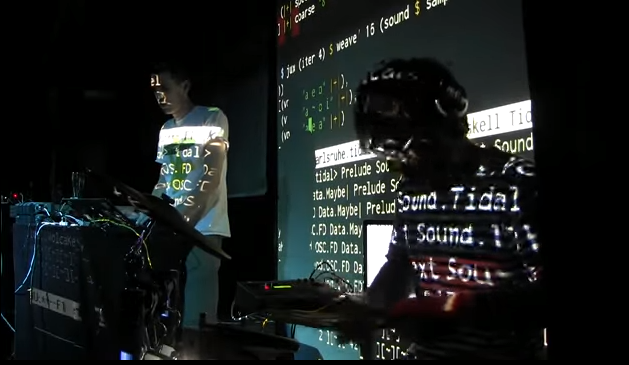
\includegraphics[scale=0.5]{imagens/canute.png}
  \caption{Performance do duo Canute (Karlesruhe, 2015) \textbf{Fonte}: \citeonline{mclean_canute_2015}.}
  \label{fig:canute}
\end{figure}
\end{frame}

% ----------------- NOVO SLIDE --------------------------------
\begin{frame}{Algorave}
\begin{figure}[h]
  \centering
  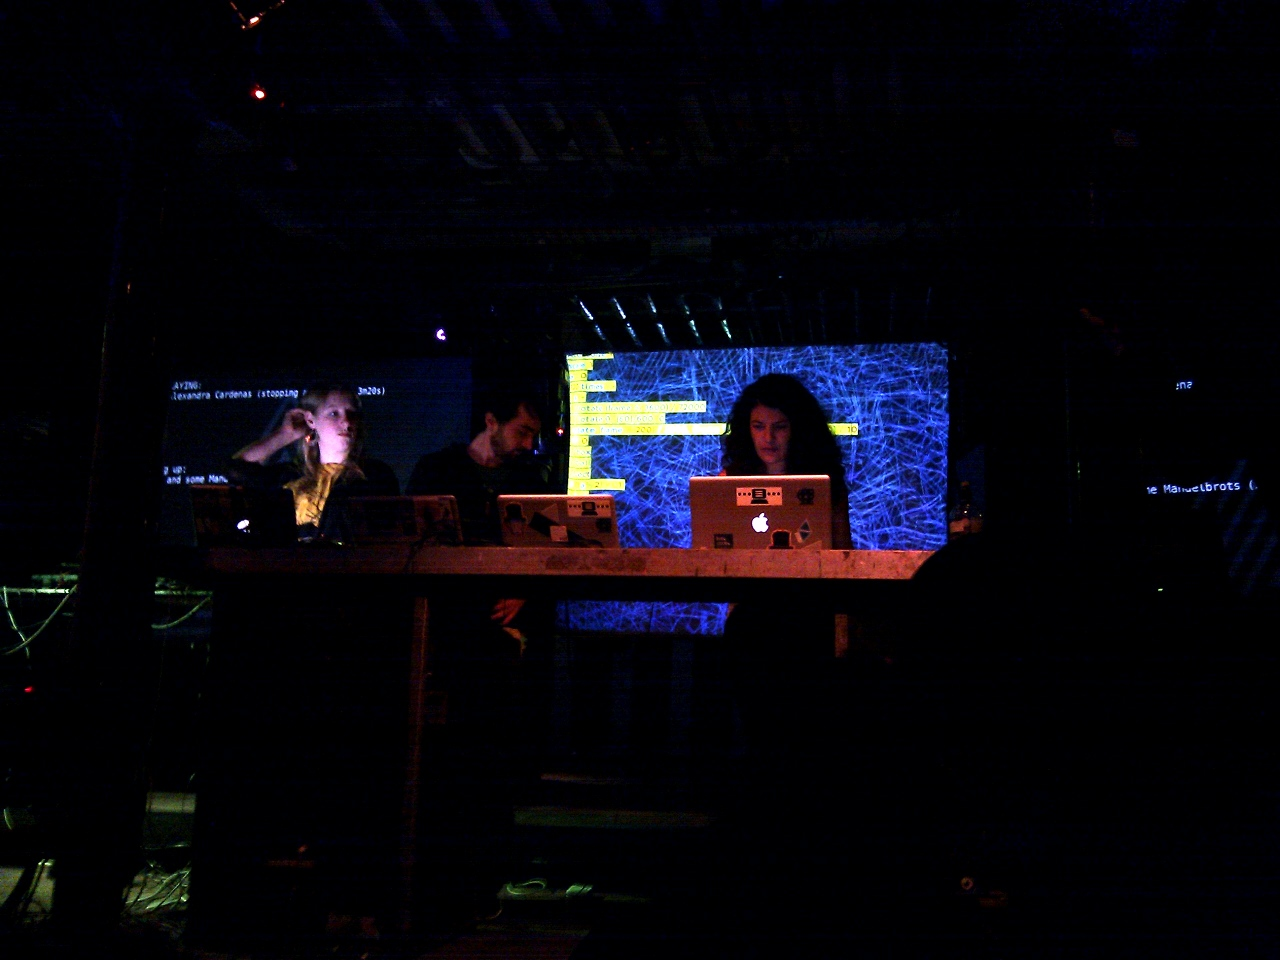
\includegraphics[scale=0.2]{imagens/cardenas.jpg}
  \caption{Performance de Alexandra Cárdenas (Londres, 2013) \textbf{Fonte}: \citeonline{griffths_algorave_2013}.}
  \label{fig:cardenas}
\end{figure}
\end{frame}

% ----------------- NOVO SLIDE --------------------------------
\begin{frame}{Algorave}
\begin{figure}[!h]
  \centering
  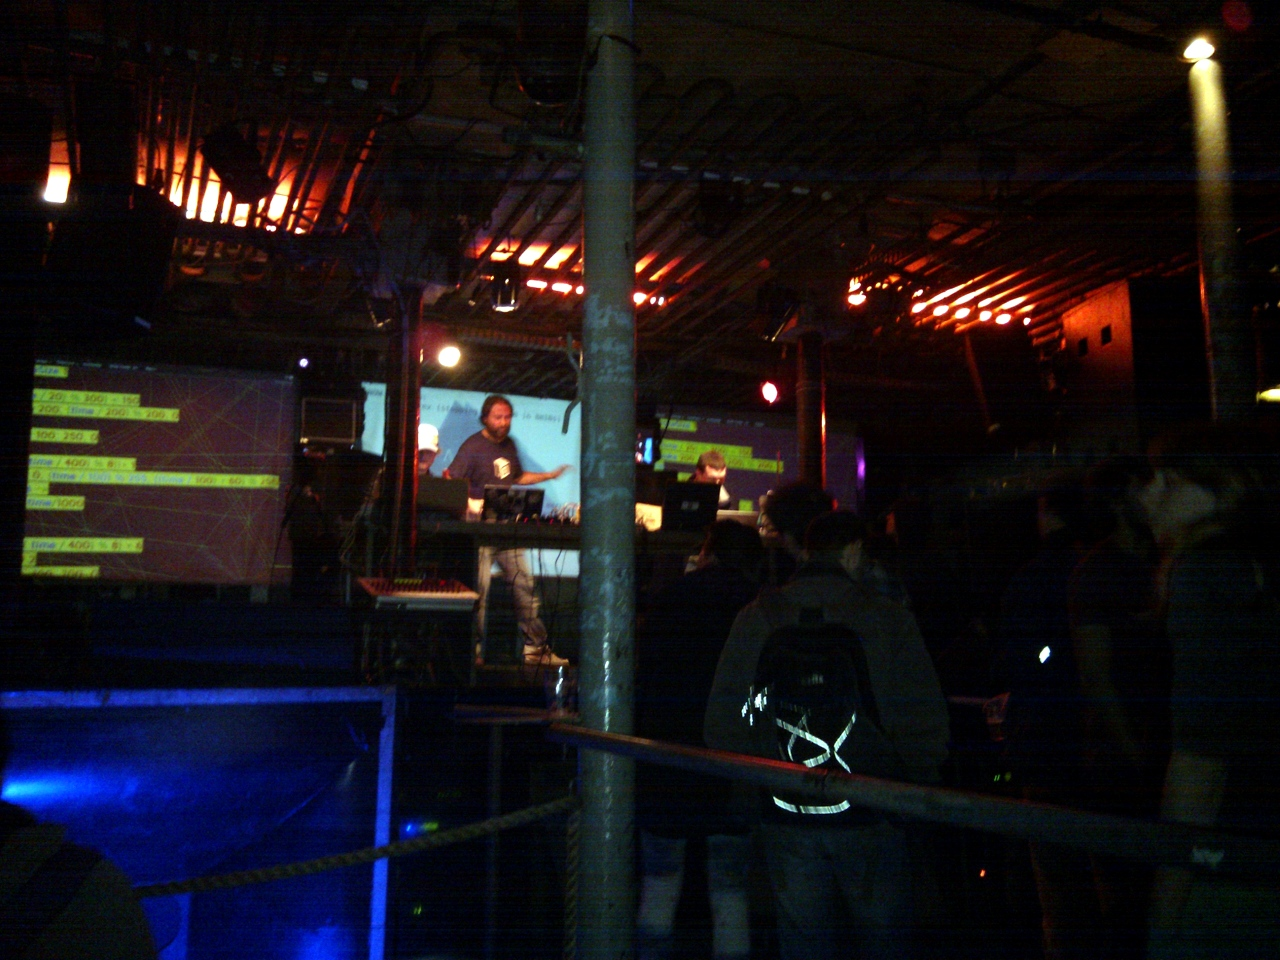
\includegraphics[scale=0.2]{imagens/algorave.jpg}
  \caption{Performance do duo Mico Rex (Londres, 2013) \textbf{Fonte}: \citeonline{griffths_algorave_2013}.}
  \label{fig:micorex}
\end{figure}
\end{frame}

% ----------------- NOVO SLIDE --------------------------------
\begin{frame}{Coreografia}
Kate Sichio

• \emph{Hacking the Body}/\emph{Hacking Choreography};

• \emph{Hacking Coreography} \emph{v.01} e \emph{v.02});

• \emph{Hacking The Body 2.0};
\end{frame}

% ----------------- NOVO SLIDE --------------------------------
\begin{frame}{Coreografia}
Para \citeonline[cap.~1, p.~3]{downie_choreography_2005}, do ponto de vista computacional, a partitura coreográfica é mais próxima do código escrito em uma linguagem de computador do que a partitura musical tradicional. 
\end{frame}

% ----------------- NOVO SLIDE --------------------------------
\begin{frame}{Coreografia}
• Assimilação do pensamento algorítmico na Dança $\rightarrow$ \emph{Sensibilidades Computacionais} \apud[cap.~1, p.~3;p.~31]{downie_choreography_2005}{sichio_hacking_2004} 

• \emph{mecanismos de generalização e abstração, representação da coreografia e dança como computação} \cite[cap.~1, p.~2--4]{downie_choreography_2005} $\rightarrow$ estratégias elaboradas por coreógrafos como Merce Cunningham, Trisha Brown, Bill T. Jones, e William Forsythe.
\end{frame}

% ----------------- NOVO SLIDE --------------------------------
\begin{frame}{Coreografia}
\emph{Esta sensibilidade computacional é presente em dois níveis em um trabalho destes coreógrafos. Primeiramente, em seus processos coreográficos -- os sistemas, métodos, e notação através dos quais os coreógrafos criam a dança. Segundo, no trabalho ele mesmo, finalizado, que aparece no palco e é interpretado pelo observador. As primeiras invenções e proclamoções de Cunningham -- a democracia do espaço do palco, e a redescoberta do que está atrás do dançarino como ponto de origem do movimento -- pode ser interpretado como generalizações do tipo; qualquer ponto do palco é a ``frente'', e conectado por um conjunto de articulações pode ser pensado como um membro. O que eram constantes, uma vez especificados em uma descrição rígida, se tornam variáveis em uma estrutura generativa.}\cite[cap.~1, p.~2--4]{downie_choreography_2005}
\end{frame}

% ----------------- NOVO SLIDE --------------------------------
\begin{frame}{Hacking Coreography}
Duas experiências com uma Partitura de Eventos do artista Alison Knowles (mais especificamente a peça de performance \#8, de 1965)
\end{frame}

% ----------------- NOVO SLIDE --------------------------------
\defverbatim{\oito}{
\scriptsize \begin{verbatim}
Divida uma variedade de objetos em dois grupos. 
Cada grupo é rotulado com "tudo". 
Estes grupos podem incluir diversas pessoas. 
Existe uma terceira divisão do palco, objetos vazios, rotulados com "nada". 
Cada um dos objetos é "alguma coisa". 
Um executante combina e ativa os objetos das seguintes maneiras para qualquer duração 
   desejada de tempo :

* "alguma coisa" com "tudo"

* "alguma coisa" com "nada"

* "alguma coisa" com "alguma coisa"

* "tudo" com "tudo"

* "tudo" com "nada"

* "nada" com "nada"
\end{verbatim}
}

\begin{frame}{Hacking Coreography}
\oito
\end{frame}

\begin{frame}{Hacking Coreography v.01}
\emph{Depois que a partitura foi completada, contudo, ela foi \emph{hackeada}. Isso significa que o executante tenta de alguma forma contornar as instruções originais. Isto foi feito sem preparações prévias e a audiência assistiu isso se desdobrar enquanto era realizada. Nesta primeira performance, o papel e os rótulos foram rasgados para criar novas palavras e categorias (\ldots) Então ao invés de ``nada''$[$Nothing$]$, foram formados dois grupos, ``não''$[$No$]$ e ``coisa''$[$Thing$]$.} \cite[p.~31]{sichio_hacking_2004}
\end{frame}

\begin{frame}{Hacking Coreography v.02}
Orientações são escritas como um híbrido de texto discursivo, legível por um executante, e de código de computador em linguagem Java. Isto é, ele não é executável por um computador para resultar em sons, mas por um humano para resultar em movimentos.
\end{frame}

\begin{frame}{Hacking Coreography v.02}
Orientações são escritas como um híbrido de texto discursivo, legível por um executante, e de código de computador em linguagem Java. Isto é, ele não é executável por um computador para resultar em sons, mas por um humano para resultar em movimentos.
\end{frame}

\defverbatim{\danca}{
\begin{minted}[fontsize=\scriptsize]{java}
/Dance/
set up()
{
dance a centre, right
dance b centre, left
}

movement()
{
move1 (dance a = rotate) (dance b = jump)
move2 (dance a = brush) (dance b = lie down)
move3 (dance a = push) (dance b = run)
move4 (dance a = step) (dance b = kneel)
}

coreography()
{
if (dancer a = rotate right 180)
then both jump = 2 feet to 1
if (dancer b = travels)
then brush = right foot
}

run(){
move1
move4
move4
move1
move2
move3
move1
move2
move3
move4
}

/hack/
{
if (dancer a = kneel)
dancer a = kneel
if (dancer a = rotate)
dancer b = rotate opposite direction 
}
\end{minted}
}

\begin{frame}[allowframebreaks]{Hacking Coreography v.02}
\danca
\end{frame}

\begin{frame}[allowframebreaks]{Hacking The Body}
\emph{Esta peça é uma exploração de eletrônica codificada ao vivo e movimentos improvisados. Uma dançarina veste uma peça de atuadores hápticos. Estes atuadores são programados em tempo-real via OSC\footnote{N.A.: ``\emph{Open Sound Control} é um protocolo de comunicação entre computadores, sintetizadores sonoros e outros dispositivos multimídia que são otimizados para as modernas tecnologias de rede''. Disponível em \url{http://opensoundcontrol.org/introduction-osc}} para 'zunir' sobre os lados direito e esquerdo da dançarina para indicar qual lado do corpo a dançarina deve mover. A partitura é codificada ao vivo pela coreógrafa enquanto a dançarina responde por uma retroalimentação háptica. Esta peça explora o \emph{live coding} de corpos, e movimento como saída, ao invés de saídas sonoras ou visuais como encontrado em muitas execuções de \emph{live coding}
}

\begin{figure}[!h]
  \centering
  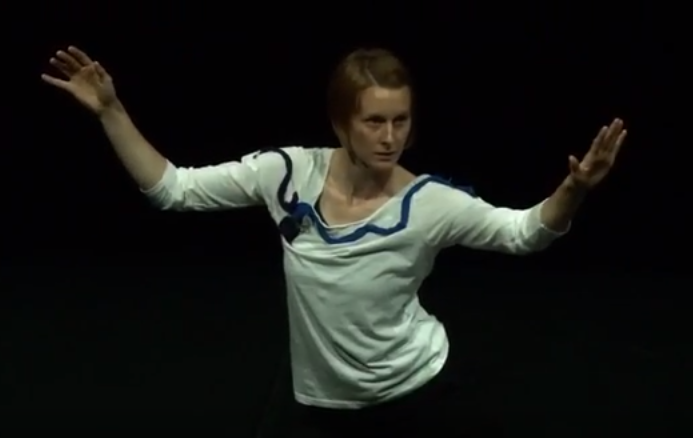
\includegraphics[scale=0.3]{imagens/iclcdanca.png}
  \caption{Dançarina (anônima) controlada por Kate Sicchio (2015) através de uma codificação improvisada. \textbf{Fonte}: \url{https://www.youtube.com/watch?v=uAq4BAbvRS4}.}
  \label{fig:iclcdanca}
\end{figure}
\end{frame}

\begin{frame}{Música computacional}
• FooBarBaz      (Aspecto histórico, em um evento nacional)

• Magno Calliman (Aspecto performático, em um evento nacional)

• Supercopair    (Aspecto telemático, com pesquisadores brasileiros)
\end{frame}

\defverbatim{\chuck}{
\begin{minted}[fontsize=\scriptsize]{c}
["samples/fx/s20.wav"] @=> Foo.name;
[0.] @=> Foo.prop;
[.25, .15] @=> Foo.rate;
[2., 1., 1., 4.] @=> Foo.du;
[.8] @=> Foo.gain;
\end{minted}
}

\begin{frame}[allowframebreaks]{Foo Bar Baz}
FooBarBaz é um grupo de improvisação de códigos formado por Gilson Beck, Renato Fabbri, Ricardo Fabbri e Vilson Vieira. Sua primeira apresentação foi durante o Festival Contato 2011. Os membros são ativos em um laboratório virtual conhecido como \emph{labMacambira}(\url{http://labmacambira.sourceforge.net/}).

\begin{figure}[!h]
  \centering
  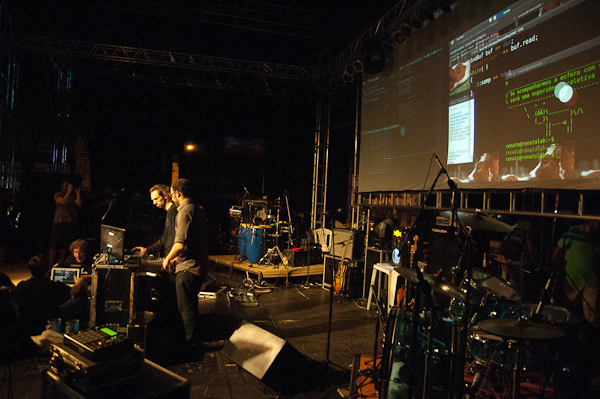
\includegraphics[scale=0.45]{imagens/Foobarbaz1.jpg}
  \caption{Festival Contato, 2011. \textbf{Fonte}: \citeonline{fabbri_wiki_2011}.}
  \label{fig:foobarbaz}
\end{figure}
\end{frame}

\begin{frame}{Foo Bar Baz}
\chuck
\end{frame}


\begin{frame}{Foo Bar Baz}
Funcionamento $\rightarrow$ \emph{grade temporal} (TimeGrid) $\rightarrow$  Graham Coleman (\url{http://www.dtic.upf.edu/~gcoleman/}).
\end{frame}

\defverbatim{\timegrid}{
\begin{minted}[fontsize=\scriptsize]{c}
//basic timing operations abbreviated

public class TimeGrid {

    dur beat;
    dur meas;
    dur sect;

    int nbeat;
    int nmeas;

    //phase and magnitude of offset
    float measPhase;
    dur measOffset;
    ...

    //sync to beat
    fun void sync() {
        beat - (now % beat) => now;
    }

    fun void sync(dur T) {
        T - (now % T) => now;
    }

    //how long to sync to this duration
    fun dur syncDur(dur T) {
	return (T - (now % T));
    }

    //minimum time
    fun dur tmin(dur a, dur b) {
	return (a < b) ? a : b;
    }
    ...
}
\end{minted}
}  

\begin{frame}[allowframebreaks]{Foo Bar Baz}
\timegrid
\end{frame}

\begin{frame}[allowframebreaks]{screenBashing}
Performance de \emph{screenBashing} de Magno Caliman (ver \autoref{fig:screenbashing}), realizada durante o XIII ENCUN\footnote{Encontro Nacional de Compositores Universitários em Campinas-SP no ano de 2015.}. 

\begin{figure}[!h]
  \centering
  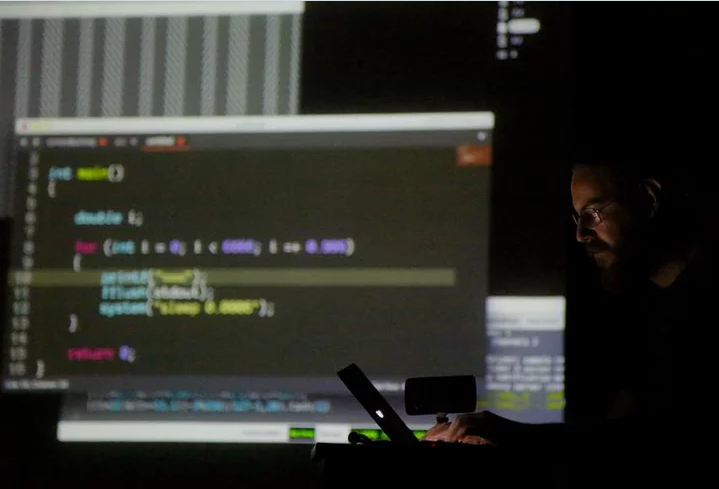
\includegraphics[scale=0.5]{imagens/screenbashing.png}
  \caption{Performance de \emph{screenBashing}. \textbf{Fonte}: \url{https://vimeo.com/148626379}.}
  \label{fig:screenbashing}
\end{figure}
\end{frame}

\begin{frame}{screenBashing}
\emph{Não acho totalmente adequado considerar como puramente um improviso. (\ldots) acredito que se imaginarmos um \emph{continuum}, uma linha onde de um lado vc tem uma improvisação totalmente livre (impossível de se alcançar, claro) e do outro uma composição 100\% determinada (tão impossível quanto), acredito que \emph{screenBashing} está posicionada mais à direita\ldots}
\end{frame}

\defverbatim{\magnoA}{
\begin{minted}[fontsize=\scriptsize]{c}
# include <stdio.h>

int main()
{
  double i;
  
  for (int i=0; i<; i < 6666; i=+0.999)
  {
      printf("\\\\    //  \\");
      fflush(stdout)
      system("sleep 0.0006")
  }
}
\end{minted}
}

\defverbatim{\magnoB}{
\begin{minted}[fontsize=\scriptsize]{bash}
# gcc - compilador
# a.c - arquivo em linguagem c
# -o  - escreve o resultado em um outro arquivo
# a   - arquivo binario alvo
\$> gcc a.c -o a
magno.c: In function 'main':
magno.c:7:12: error: conflicting types for 'i'
\end{minted}
}

\defverbatim{\magnoC}{
\begin{minted}[fontsize=\scriptsize]{bash}
\\\\    //  \\\\\\    //  \\\\\\    //  \\\\\\    //  \\\\\\    //
  \\\\\\    //  \\\\\\    //  \\\\\\    //  \\\\\\    //  \\\\\\  
  //  \\\\\\    //  \\\\\\    //  \\\\\\    //  \\\\\\    //  \\\\
\\    //  \\\\\\    //  \\\\\\    //  \\\\\\    //  \\\\\\    //  
\\\\\\    //  \\\\\\    //  \\\\\\    //  \\\\\\    //  \\\\\\    
//  \\\\\\    //  \\\\\\    //  \\\\\\    //  \\\\\\    //  \\\\\\
    //  \\\\\\    //  \\\\\\    //  \\\\\\    //  \\\\\\    //  \\\
\\\    //  \\\\\\    //  \\\\\\    //  \\\\\\    //  \\\\\\    //  
\\\\\\    //  \\\\\\    //  \\\\\\    //  \\\\\\    //  \\\\\\    /
/  \\\\\\    //  \\\\\\    //  \\\\\\    //  \\\\\\    //  \\\\\\  
  //  \\\\\\    //  \\\\\\    //  \\\\\\    //  \\\\\\    //  \\\\\
\    //  \\\\\\    //  \\\\\\    //  \\\\\\    //  \\\\\\    //  \\
\\\\    //  \\\\\\    //  \\\\\\    //  \\\\\\    //  \\\\\    /
\end{minted}
}  

\begin{frame}[allowframebreaks]{screenBashing}
Código-fonte:

\magnoA

Execução:

\magnoB

Resultado:

\magnoC
\end{frame}

\begin{frame}{screenBashing}
• O código sonoro foi pouco exposto

• Valorização ideológica. $\rightarrow$ repetição dos algarismos seis e nove $\rightarrow$ \emph{black metal} abstrato (?) 

• uma segunda notação (Capítulo 3), mais enxuta e sem erros, permite apontar a questão ideológica
\end{frame}

\defverbatim{\magnoD}{
\begin{minted}[fontsize=\scriptsize]{c}
# include <stdio.h>
int main(){
  int i=0;
  for (;;i++){
      printf("=====  ______");
      fflush(stdout);
      // 30 frames por segundo 
      // ou um limite aproximado da
      // pecepcao humana (1/30)
      system("sleep 0.033");
  }
}
\end{minted}
}  

\defverbatim{\magnoE}{
\begin{minted}[fontsize=\scriptsize]{bash}
=====  ______=====  ______=====  ______=====  ______=====  ______=====
  ______=====  ______=====  ______=====  ______=====  ______=====  ___
___=====  ______=====  ______=====  ______=====  ______=====  ______==
===  ______=====  ______=====  ______=====  ______=====  ______=====  
______=====  ______=====  ______=====  ______=====  ______=====  _____
_=====  ______=====  ______=====  ______=====  ______=====  ______====
=  ______=====  ______=====  ______=====  ______=====  ______=====  __
____=====  ______=====  ______=====  ______=====  ______=====  ______=

\end{minted}
}

\begin{frame}{screenBashing}
Código-fonte:

\magnoD

Resultado:

\magnoE
\end{frame}

\begin{frame}{Telepresença e espaços virtuais}
• Uma rede local, com computadores diferentes, mas com os improvisadores fisicamente próximos;

• Uma rede remota, privada, que comunica um conjunto de pessoas fisicamente distantes \citeonline[p.~152--153]{junior_supercopair_2015}

• O navegador de \emph{internet} se torna o ambiente virtual de criação musical \cite{roberts_web_2013}.
\end{frame}

\begin{frame}{Telepresença e espaços virtuais}
\emph{live coding sessions} $\rightarrow$ sessões de improvisações que ocorrem em encontros, simpósios e \emph{workshops}, ricamente documentadas (\url{https://supercollider.github.io/archive}).
\end{frame}

\begin{frame}{Telepresença e espaços virtuais}
Performance telepresencial em 2014, por Ben Swift, Henry Gardner e Andrew Sorensen, realizada entre dois intérpretes-programadores localizados na Alemanha e Estados Unidos usando um servidor SSH localizado na Australia \cite[p.~152--153]{junior_supercopair_2015}
\end{frame}

\begin{frame}{Telepresença e espaços virtuais}
\emph{Supercopair} (\url{https://github.com/deusanyjunior/atom-supercopair}) $\rightarrow$ ambiente cooperativo de improvisação de códigos.
\end{frame}

\begin{frame}{Telepresença e espaços virtuais}
Execuções remotas em navegadores de \emph{internet}, com auxílio da biblioteca \emph{WebAudio API} (\url{https://dvcs.w3.org/hg/audio/raw-file/tip/webaudio/specification.html}).
\end{frame}

\begin{frame}{Telepresença e espaços virtuais}
• \emph{Gibber} \cite{roberts_gibber:_2012} (\url{http://gibber.mat.ucsb.edu/}); 

• \emph{Wavepot}(\url{http://www.wavepot.com});

• \emph{Vivace} \cite{vieira_vivace:_2015} (\url{http://void.cc/freakcoding})

• \emph{Termpot} \cite{lunhani_termpot_2015} (\url{http://jahpd.github.io/termpot})
\end{frame}

\section{Definições Históricas da Improvisação de códigos}
\begin{frame}{Definições Históricas da Improvisação de códigos}
Exemplos proto-históricos $\rightarrow$ possuem similaridades com o conjunto de regras práticas publicadas por \cite{ward_live_2004}
\end{frame}


\begin{frame}{Definições Históricas da Improvisação de códigos}
• Pietro Grossi
  
• Baía de São Franscisco
\end{frame}

\begin{frame}{Definições Históricas da Improvisação de códigos}
Evento Histórico: Live Algorithm Programming and Temporary Organization for its Promotion
\end{frame}

\begin{frame}{Pietro Grossi -- Computer Concerto}
\emph{Grossi começou a se interessar por música computacional durante a primeira metade doas anos 60, quando ele quando ele organizou um programa de rádio centrado em torno da "música inovadora" em geral \cite{giomi_conversasioni_1999}. Contudo a primeira experiência de Grossi com um computador foi em Milão, no Centro de Pesquisa Elétrica da Olivetti-General. Aqui, auxiliado por alguns técnicos internos e engenheiros, ele conseguiu compor e gravar alguns de seus primeiros trabalhos em música computacional. Eles foram, em sua maior parte, transcrições de música clássica ocidental. Contudo, houve algumas exceções, por exemplo, uma faixa chamada Mixed Paganini} \cite[p.~126]{mori_pietro_2015}
\end{frame}

\begin{frame}{Pietro Grossi -- DCMP (\emph{Digital Computer Music Program})}
\emph{Um dos mais importantes aspectos do trabalho de Grossi foi que todas intervenções eram instantâneas: o operador não tinha que esperar pelo computador terminar todas operações requisitadas, e depois ouvir os resultados. Cálculos de dados e reprodução sonoras eram simultâneos. \textbf{Esta simultaneidade não era comum no campo da \emph{Computer Music} daquele tempo, e Grossi deliberadamente escolheu trabalhar desta forma, perdendo muito no lado da qualidade sonora. Seu desejo era poder escutar os sons resultantes imediatamente}} \cite[p.~126]{mori_pietro_2015}
\end{frame}

\begin{frame}{Pietro Grossi -- DCMP (\emph{Digital Computer Music Program})}
``preguiçoso'' (\emph{pigro}, \emph{lazy}) $\rightarrow$ \emph{reflexividade}
\end{frame}

\begin{frame}{Pietro Grossi -- DCMP (\emph{Digital Computer Music Program})}
\emph{habilidade de um programa manipular como dados algo que representa o estado do programa durante sua própria execução, o mecanismo para codificação de estados de execução é chamado \emph{reificação}}.\cite[p.~1]{malefant_reflection_1996}.
\end{frame}

\begin{frame}{Pietro Grossi -- DCMP (\emph{Digital Computer Music Program})}
\emph{Naquele tempo, os recursos de cálculo eram escassos e, para obter a reprodução em tempo-real citada, era necessário pedir por pouca quantidade de dados. (\ldots) A síntese de timbres necessita de uma quantidade imensa de dados, e então a escolha foi descartá-la temporariamente, e todos os sons eram reproduzidos com o timbre de uma onda quadrada. Esta forma de onda era gerada por extração do estado binário do \emph{pin} de saída da placa mãe que controla o programa. Essa saída tinha um único \emph{bit}, e então a onda sonora gerada era o resultado desta mudança do estado binário. Desta forma, o computador não emprega quaisquer recursos para calcular a síntese sonora, economizando-os para o processo de produção musical. Grossi não estava interessado na qualidade da saída sonora em sua primeira fase em Pisa. O que importava particularmente era a capacidade em trabalhar em tempo real, ou, em outras palavras, para ter a escolha de escutar imediatamente ao que ele escreveu no teclado do terminal de vídeo} \apud{giomi_conversasioni_1999}{mori_pietro_2015}.
\end{frame}

\begin{frame}{Pietro Grossi -- TAU2-TAUMUS (\emph{Terminale Audio 2$^a$ versione)}}
Grossi foi capaz de implementar melhorias de timbre, digitalmente controladas por doze vozes, com síntese analógica.
\end{frame}

\begin{frame}{Pietro Grossi -- TAU2}
\emph{Estas doze vozes eram divididas em três grupos, compostos de quatro canais cada. O operador poderia atribuir um timbre diferente para cada grupo, que era modulado usando síntese aditiva com sete sobretons. Cada sobretom era controlado individualmente pelo programa.}
\end{frame}

\begin{frame}{Pietro Grossi -- TELETAU}
O TAU2-TAUMUS sofreu uma considerável modificação, sendo que era possível controlar o sistema digital-analógico remotamente. O novo programa foi batizado de TELETAU \citeonline[p.~128--129]{mori_pietro_2015}
\end{frame}

\begin{frame}{Pietro Grossi -- TELETAU}
\emph{Grossi fez sua primeira experiência do tipo durante uma conferência de tecnologia em Rimini em 1970, onde o músico reproduzia algumas de suas composições, bem como sons randômicos, empregando um terminal de vídeo conectado pelo telefone para o computador da CNR em Pisa. A RAI, empresa de radiodifusão italiana, emprestou suas pontes de rádio $[$Comunicação entre duas antenas$]$ para enviar sinais sonoros entre Pisa e Rimini. É como se fosse o primeiro experimento de telemática musical no mundo} \cite[p.~129]{mori_pietro_2015}.
\end{frame}

\begin{frame}{Baía de São Franscisco}
• The League of Automatic Composers

• The Hub

• Ron Kuivilla
\end{frame}

\begin{frame}{Baía de São Franscisco}
\emph{Mills College} em Oakland. 
\end{frame}

\begin{frame}{Baía de São Franscisco}
\emph{Com o florescimento da indústria de computadores pessoais na Baía de São Franscisco, o acesso às novas tecnologias e pessoas que desenvolveram elas era talvez o melhor no mundo. (\ldots) Esta também é a cultura que deu ao mundo a música ``New Age'', uma versão aguada e comercializada das músicas com base em modos e drones que Terry Riley, Pauline Oliveros, e LaMonte Young inventaram durante os anos cinquenta e sessenta. Mas a música feita na Costa Oeste também incluiam improvisações barulhentas e livre de restrições, que sobraram das revoluções contra-culturais dos anos 60}\cite{brown_indigenous_2013}.
\end{frame}

\begin{frame}{The League of Automatic Composers}
• Segunda metade da década de setenta: Jim Horton começa a adquirir micro-controladores KIM-1 (\emph{Keyboard Input Monitor}, \url{http://www.6502.org/trainers/buildkim/kim.htm}), com interesses musicais. 

• David Behrman e John Bischoff, Rich Gold, Cathy Morton, Paul Robinson, e Paul Kalbach.
\end{frame}

\begin{frame}{KIM1}
\begin{figure}[!h]
  \centering
  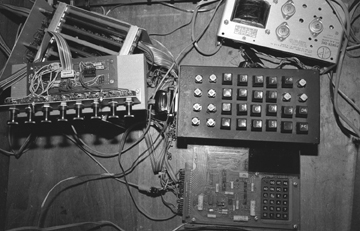
\includegraphics[scale=0.7]{imagens/siskim1.jpg}
  \caption{Sistema de música computacional de John Bischof \emph{circa} 1980. Foto: Eva Shoshanny\protect\footnotemark. \textbf{Fonte}: \citeonline{brown_indigenous_2013}.}
  \label{fig:siskim1}
\end{figure}
\end{frame}

% ----------------- NOVO SLIDE --------------------------------
\section*{Referências}

% --- O comando \allowframebreaks ---
% Se o conteúdo não se encaixa em um quadro, a opção allowframebreaks instrui 
% beamer para quebrá-lo automaticamente entre dois ou mais quadros,
% mantendo o frametitle do primeiro quadro (dado como argumento) e acrescentando 
% um número romano ou algo parecido na continuação.

\begin{frame}[allowframebreaks]{Referências}
\bibliography{main}
\end{frame}

% ----------------- FIM DO DOCUMENTO -----------------------------------------
\end{document}
